\documentclass{beamer}

\usepackage[francais]{babel}
\usepackage[T1]{fontenc}
\usepackage[latin1]{inputenc}
\usepackage{listings}
\usepackage{graphicx}
\usepackage{multicol}
\usepackage{changepage}

\newcommand{\putat}[3]{\begin{picture}(0,0)(0,0)\put(#1,#2){#3}\end{picture}}

\usetheme{Warsaw}

\newif\ifplacelogo %Bool�en pour placer ou non le logo
\placelogotrue %Initialisation bool�en � 'True'
\logo{\ifplacelogo
\includegraphics[height=5mm]{LogoINSA.png}\fi} %Initialisation du logo (fonction du bool�en)

\title{Projet Math�matiques}
\subtitle{L'interpolation par spline}
\author[OB \--- CG \--- ASM \--- BP \--- DT ]{Olivia BRIODEAU \\ Caroline GOUMENT \\ Andrei-Silviu MILEA\\ Bozhidar PALASHEV \\  Damien TOOMEY}
\institute[ ]{INSA de Rouen}
\date{\today}

\begin{document}
	
	\begin{frame} 
		\titlepage
	\end{frame}
		
		
		
	\placelogofalse
	\begin{frame}[label=sommaire] 
		\frametitle{Sommaire} 
     	    \begin{multicols}{2}
    		\tableofcontents
    		\end{multicols}
	\end{frame}	
	
	\placelogotrue
	\section{Introduction}
	\begin{frame} 
		\frametitle{Introduction}
		\begin{alertblock}{Les domaines o\`u on emploie le mot 'interpolation'}
			\begin{itemize}
				\item Musique 
				\item Graphique
				\item Informatique
				\item Math\'ematiques	
				\item M\'ethodologie
				\item Industrie de film et d'animation
			\end{itemize}
		\end{alertblock}
		\hyperlink{sommaire}{\beamerreturnbutton{Retour Sommaire}}
	\end{frame}
	
	
	
	\placelogotrue
	\section{Point historique}
		\subsection{Interpolation}
	\begin{frame} 
		\frametitle{Interpolation}
		\begin{alertblock}{Grands Points}
		
			\begin{itemize}
				\item Babyloniennes, Indiens, Chinois
				\item Newton 1711
				\item Gregory-Newton, Newton-Gauss, Stirling-Newton
				\item Lagrange $18^{eme}$ si\`ecle
				\item $19^{eme}$ si\`ecle Gauss, Bessel et Cauchy
				\item fin $19^{eme}$ si\`ecle innovations de Tchebychef et Hermite
			\end{itemize}
		\end{alertblock}
		\begin{figure}
		\putat{95}{45}
				{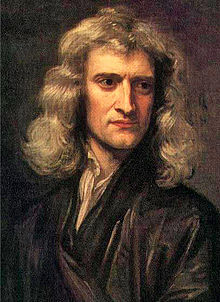
\includegraphics[width=0.2\textwidth]{Newton.jpg}}
		\end{figure}
		\hyperlink{sommaire}{\beamerreturnbutton{Retour Sommaire}}
	\end{frame}
	
	
	
	\placelogotrue
	\subsection{Splines}
	\begin{frame} 
		\frametitle{Splines}
		\begin{alertblock}{Grands points}
		\begin{itemize}
			\item conception et fabrication des bateaux
			\item travail avec des dispositifs � ducks �
			\item 1940 Shanon et Schoenberg, les principales fondateurs 
			\item $19^{eme}$ si\`ecle apparition des ordinateurs :\\ construction -> tracer des courbes
			\item industrie a�ronautique Boeing, British Aircraft Corporation
			\item industrie automobile Renault, Citro�n, General Motors
		\end{itemize}	
		\end{alertblock}
    	\hyperlink{sommaire}{\beamerreturnbutton{Retour Sommaire}}
	\end{frame}
	
	
	
	
	\placelogofalse
	\section{Courbes de B\'ezier }
		\subsection{Contexte}
	\begin{frame} 
		\frametitle{Contexte}
		
		\begin{alertblock}

			Context
		\end{alertblock}
		
		\begin{figure}
				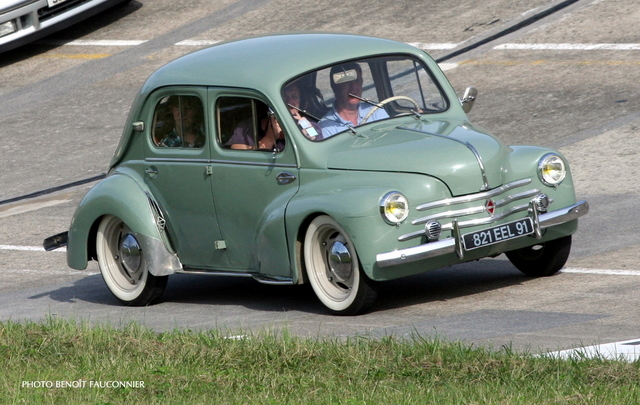
\includegraphics[width=0.5\textwidth]{renault_4.jpg}
		\end{figure}
		
		\begin{alertblock}
		
			Unisurf
		\end{alertblock}
		
		\hyperlink{sommaire}{\beamerreturnbutton{Retour Sommaire}}
	\end{frame}
	

	
	
	\placelogofalse	
		\subsection{Partie Math\'ematiques}
	\begin{frame} 
		\frametitle{Partie Math\'ematiques}
		\begin{exampleblock}

 			\[\begin{pmatrix}
				A' \\
				B' \\
				C' \\ 
				D'\\
				\end{pmatrix}
				=
				\begin{pmatrix}
				1 & 0 & 0 & 0 \\[5pt]
				\frac{1}{2} & \frac{1}{2} & 0 & 0 \\[5pt]
				\frac{1}{4} & \frac{2}{4} & \frac{1}{4} & 0 \\[5pt]
				\frac{1}{8} & \frac{3}{8} & \frac{3}{8} & \frac{1}{8} \\[5pt]
				\end{pmatrix}
				\begin{pmatrix}
				A \\
				B \\
				C \\ 
				D \\
			\end{pmatrix}\]\\
			
			\[B_{i, n} (t) = \dbinom{n}{i}t^i(1-t)^{n-i}\]
			
		\end{exampleblock}
		\begin{alertblock}{Forme g\'en\'erale de la coube de B\'ezier cubique}
		$B(t) = P_0 (1-t)^3 + 3P_1 t(1-t)^2 + 3P_2 t ^2 (1-t) + P_3 t^3 , \qquad t \in [0,1]$
		\end{alertblock}
    	\hyperlink{sommaire}{\beamerreturnbutton{Retour Sommaire}}
	\end{frame}
	
	
	
	
\placelogofalse
	\section{Splines cubiques}
		\subsection{Exemple de calcul d'une fonction spline cubique}
	\begin{frame}

	  
		\frametitle{Exemple de calcul d'une fonction spline cubique}
Consid�rons les 5 points ($x_i$,$f_i$) suivants : (1;6),(2;3),(3;0),(4;2),(5;6).
\\[5pt]
\underline{1\`{e}re \'{e}tape : on remplace les coefficients dans la matrice A}
\\[5pt]
$h_i=x_{i+1}-x_i$
\\
Ici, $h_i=1$ pour $i = 0,...,3$
\begin{adjustwidth*}{-2cm}{-2cm}
\[A= \begin{pmatrix}
1 & 0 & 0 & 0 & 0 \\
h_0 & 2(h_1+h_0) & h_1 & 0 & 0 \\
0 & h_1 & 2(h_2+h_1) & h_2 & 0 \\
0 & 0 & h_2 & 2(h_3+h_2) & h_3 \\
0 & 0 & 0 & 0 & 1
\end{pmatrix}
= \begin{pmatrix}
1 & 0 & 0 & 0 & 0 \\
1 & 4 & 1 & 0 & 0 \\
0 & 1 & 4 & 1 & 0 \\
0 & 0 & 1 & 4 & 1 \\
0 & 0 & 0 & 0 & 1
\end{pmatrix}\]
\end{adjustwidth*}
\end{frame}



\begin{frame}
(1;6),(2;3),(3;0),(4;2),(5;6)
\\
\underline{2\`eme \'{e}tape : on simplifie notre syst\`{e}me matriciel}
\\
\begin{align*}
&\underbrace{
  \begin{pmatrix}
  1 & 0 & 0 & 0 & 0 \\
  1 & 4 & 1 & 0 & 0 \\
  0 & 1 & 4 & 1 & 0 \\
  0 & 0 & 1 & 4 & 1 \\
  0 & 0 & 0 & 0 & 1
 \end{pmatrix}
}_{A}
\underbrace{
\begin{pmatrix}
   f''_0 \\
   f''_1 \\
f''_2 \\
   f''_3 \\
f''_4 \\
 \end{pmatrix}
}_{X}
=
\underbrace{
\begin{pmatrix}
  0\\ 
6(f_{2}-2f_1+f_{0})\\
6(f_{3}-2f_2+f_{1})\\
6(f_{4}-2f_3+f_{2})\\
0
 \end{pmatrix}
}_{G}
\\[5pt]
\Leftrightarrow &\underbrace {\begin{pmatrix}
   4 & 1 & 0 \\
   1 & 4 & 1 \\
   0 & 1 & 4  
\end{pmatrix}}_{A}
\underbrace {\begin{pmatrix}
   f''_1 \\
   f''_2 \\
   f''_3 \\
\end{pmatrix}}_{X}
=
\underbrace {\begin{pmatrix}
0\\
30\\
12
\end{pmatrix}}_{G}
\end{align*}
\end{frame}

\begin{frame}
\underline{3\`{e}me \'{e}tape : On r\'{e}sout notre syst\`eme d'\'{e}quations directement ou en}
\\[2pt]
\underline{utilisant l'algorithme de Thomas}
\\[5pt]
\textbf{Algorithme de Thomas :}
\\
La r\'{e}solution du syst\`{e}me AX=G est alors ramen\'{e}e \`{a} la r\'{e}solution successive des syst\`{e}mes UX=Y et LY=G, pour ensuite avoir LUX=G, ce qui \'{e}quivaut \`a AX=G.

On a les matrices suivantes :
\[A=\begin{pmatrix}
4 & 1 & 0\\
1 & 4 & 1\\
0 & 1 & 4
\end{pmatrix}
=\begin{pmatrix}
s_1 & w_1 & 0\\
e_2 & s_2 & w_2\\
0 & e_3 & s_3
\end{pmatrix}\]
\[L=\begin{pmatrix}
1 & 0 & 0\\
\beta_2 & 1 & 0\\
0 & \beta_3 & 1
\end{pmatrix}
\qquad
U=\begin{pmatrix}
\alpha_1 & c_1 & 0\\
0 & \alpha_2 & c_2\\
0 & 0 & \alpha_3
\end{pmatrix}
\]
\end{frame}

\begin{frame}
Les relations sur les coefficients $\alpha_i$ et $\beta_i$ trouv\'{e}es dans le rapport sont :
\[\alpha_1=s_1,\; \beta_i=\frac{e_i}{\alpha_{i-1}},\; \alpha_i=s_i-\beta_{i}w_{i-1} \qquad i=2,...,n\]
Ainsi,
\[L=\begin{pmatrix}
   1 & 0 & 0 \\
   \frac{1}{4} & 1 & 0 \\
   0 & \frac{4}{15} & 1  
\end{pmatrix}
\qquad
U=\begin{pmatrix}
   4 & 1 & 0 \\
   0 & \frac{15}{4} & 1 \\
   0 & 0 & \frac{56}{15}  
\end{pmatrix}\]
\\[10pt]
On r\'{e}sout ensuite successivement les syst\`{e}mes LY=G et UX=Y.
\end{frame}

\begin{frame}
Pour \textbf{LY=G}, on pose :
$\; X=\begin{pmatrix}
   x_1 \\
   x_2 \\
   x_3  
\end{pmatrix}
\qquad Y=\begin{pmatrix}
   y_1 \\
   y_2 \\
   y_3  
\end{pmatrix}$

\begin{align*}
LY=G \;\; \Leftrightarrow \;
&\begin{pmatrix}
   1 & 0 & 0 \\
  \frac{1}{4} & 1 & 0 \\
   0 & \frac{4}{15} & 1
\end{pmatrix}
\begin{pmatrix}
   y_1 \\
   y_2 \\
   y_3  
\end{pmatrix} = \begin{pmatrix}
   0 \\
   30 \\
   12  
\end{pmatrix}
\\[5pt]
\Leftrightarrow \;  & Y= \begin{pmatrix}
0 \\
30 \\
4  
\end{pmatrix}
\end{align*}
\end{frame}

\begin{frame}
Pour \textbf{UX=Y}, on a :
$\; X=\begin{pmatrix}
   x_1 \\
   x_2 \\
   x_3  
\end{pmatrix}
\qquad Y= \begin{pmatrix}
		0 \\
		30 \\
		4  
\end{pmatrix}$
\begin{align*}
UX=Y \;\; & \Leftrightarrow \;\; \begin{pmatrix}
4 & 1 & 0 \\
0 & \frac{15}{4} & 1 \\
0 & 0 & \frac{56}{15}
\end{pmatrix}
\begin{pmatrix}
x_1 \\
x_2 \\
x_3  
\end{pmatrix} = \begin{pmatrix}
0 \\
30 \\
4  
\end{pmatrix}
\\[5pt]
&\Leftrightarrow X=\begin{pmatrix}
-\frac{27}{14} \\[5pt] 
 \;\;\;\frac{54}{7} \\[5pt] 
\;\;\;\frac{15}{14} \\[5pt] 
\end{pmatrix}
\end{align*}
Ainsi,
\\
$f''_0=0 \qquad f''_1=-\frac{27}{14} \qquad f''_2=\frac{54}{7} \qquad f''_3=\frac{15}{14} \qquad f''_4=0$
\end{frame}

\begin{frame}
\underline{4\`{e}me \'{e}tape : on calcule les splines}
\\[5pt]
\[s_i(x) = f''_i \frac{(x_{i+1}-x)^3}{6h_i}+ f''_{i+1} \frac{(x-x_i)^3}{6h_i}+a_i(x_{i+1}-x) + b_i (x-x_i)\]
\\[5pt] 
$i= 0,1,...,n-1 \;\; et \;\; h_i=x_{i+1}-x_i$
\[avec \; a_i= \frac{f_i}{h_i}-f''_i \frac{h_i}{6} \;\; et \;\; b_i= \frac{f_{i+1}}{h_i}-f''_{i+1}\frac{h_i}{6}\]
\end{frame}

\begin{frame}
Ainsi, pour les 5 points, on obtient 4 splines :
\\[10pt]
$s_0(x) = -\frac{27}{14} \frac{(x-1)^3}{6}+ 6(2-x) + \frac{93}{28}(x-1)$
\\[10pt]
$s_1(x) = -\frac{27}{14} \frac{(3-x)^3}{6} +\frac{54}{7} \frac{(x-2)^3}{6} + \frac{93}{28}(3-x) - \frac{9}{7}(x-2)$
\\[10pt]
$s_2(x) = \frac{54}{7}\frac{(4-x)^3}{6} + \frac{15}{14} \frac{(x-3)^3}{6}-\frac{9}{7}(4-x) + \frac{51}{28}(x-3)$
\\[10pt]
$s_3(x) = \frac{15}{14} \frac{(5-x)^3}{6} + \frac{51}{28}(5-x) + 6(x-4)$
\end{frame}	

\begin{frame}
			\begin{figure}
			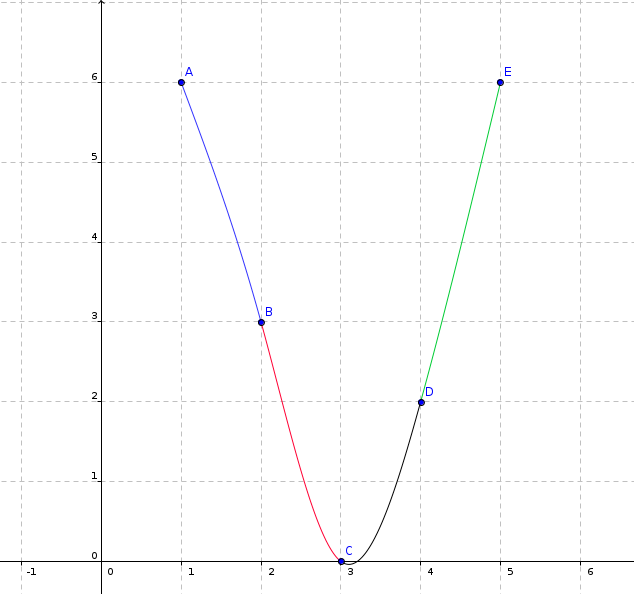
\includegraphics[width=5.8cm]{ExempleInterpolationGeogebra.png}
			\caption{Exemple d'interpolation par spline cubique sur Geogebra}
		\end{figure}
		\end{frame}	
	
	
	
	
	\placelogotrue
	\section{B-splines}
		\subsection{Les bases des B-splines}
	\begin{frame}  
		\frametitle{Les bases des B-splines}
		\begin{exampleblock}{En cas g\'en\'eral:}
    		$X_{k}(t) =\sum\limits_{i} B_{i,k}(t) . P_{i}$\\
			$B_{i,k}(t)= 
	\dfrac{t_{i+1+k}-t}{t_{i+1+k}-t_{i+1}}B_{i+1,k-1}(t) + \dfrac{t-t_{i}}{t_{i+k}-	t_{i}} B_{i,k-1}(t)$
		\end{exampleblock}
    	\hyperlink{sommaire}{\beamerreturnbutton{Retour Sommaire}}
	\end{frame}

	
	
	
	
	\placelogofalse
		\subsection{Courbe de degr\'e 3 (k=3)}
	\begin{frame}  
		\frametitle{Courbe de degr\'e 3 (k=3)}
		\begin{exampleblock}

    		Exemple de courbe de B-spline de degr\'e 3 avec points de contr\^ole $(1,1),(1,3),(2,4),(3,1)$ et vecteur n\oe ud $(1,2,3,4,5,6,7)$
		\begin{figure}
			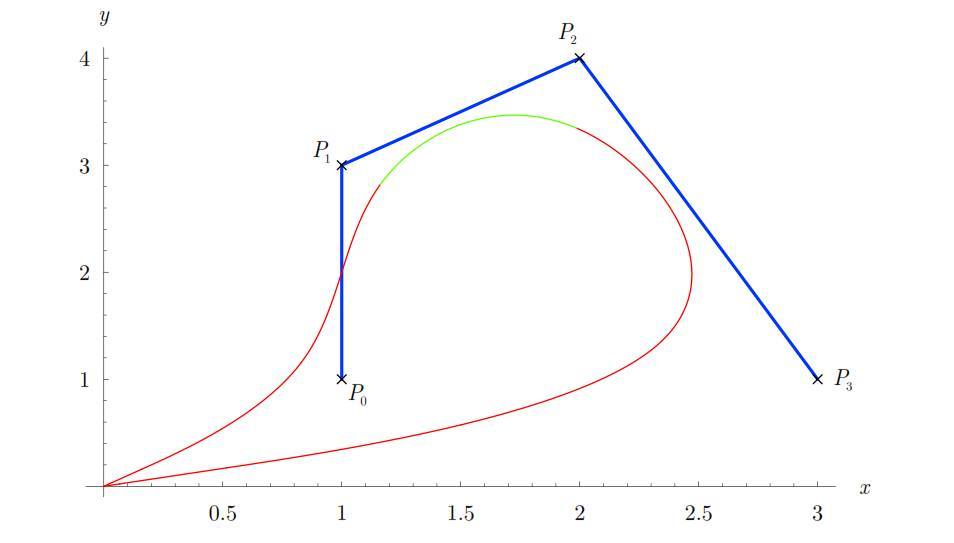
\includegraphics[width=0.7\textwidth]{Courbe-B-splines.jpg}
		\end{figure}	
		\end{exampleblock}
    	\hyperlink{sommaire}{\beamerreturnbutton{Retour Sommaire}}
	\end{frame}

	
	\section{Avantages et inconv\'{e}nients}
	\begin{frame}
	%\subsection{Courbes de B\'{e}zier}
	\begin{exampleblock}{Courbes de B\'ezier}
	\begin{itemize}
	\item AVANTAGES: Simplicit\'{e]} et description de formes complexes
	\item INCONVENIENTS: manque de contr\^{o}le local et ph\'{e}nom\ `{e}ne de Runge
	\end{itemize}	
	\end{exampleblock}
	
	%\subsection{Splines cubiques}
	\begin{exampleblock}{Splines cubiques}
	\begin{itemize}	
	\item AVANTAGES: Stabilit\'{e}, simplicit\'{e]} et courbes harmonieuses
	\item INCONVENIENTS: spline oscillante si d�riv\'{e}es trop grandes
	\end{itemize}
	\end{exampleblock}
	
	%\subsection{B-Splines}
	\begin{exampleblock}{B-splines}	
	\begin{itemize}
	\item AVANTAGES: contr\^{o}le local possible, degr\'{e} du polynome ind\'{e]}pendant du nombre de points de contr\^{o}le \\
	\item INCONVENIENTS: complexit\'{e}
	\end{itemize}
	\end{exampleblock}
	
	\end{frame}
	
	\placelogotrue
	\section{Exemples de fonctions}
		\subsection{Fonction de Runge}
	\begin{frame} 
		\frametitle{Fonction de Runge}
		\begin{alertblock}

 			1901 : Carle David Tolme Runge et le ph\'enom\`ene de Runge
		\end{alertblock}
		\begin{figure}
		\putat{-150}{-70}
			{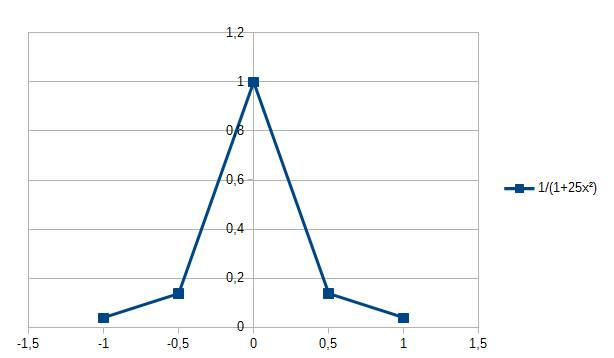
\includegraphics[width=0.5\textwidth]{CourbeFonctionRunge.png}}
		\end{figure}
		\begin{figure}
			\putat{25}{-30}
			{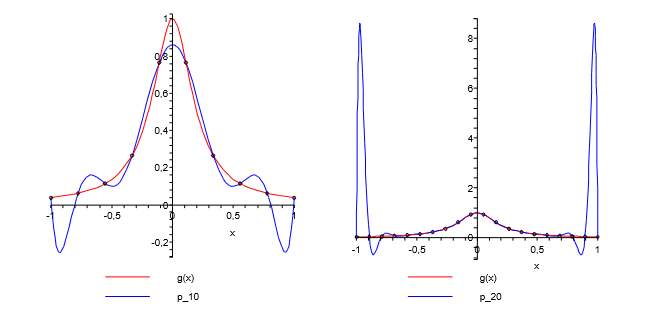
\includegraphics[width=0.5\textwidth]{ExempleFctRunge.png}}
		\end{figure}
	\end{frame}
	
	
	
	
	\placelogofalse
		\subsection{Fonctions Cosinus et Exponentielle}
	\begin{frame}  
		\frametitle{Fonctions Cosinus et Exponentielle}
		
    		\begin{figure}
    		\putat{-150}{-45}{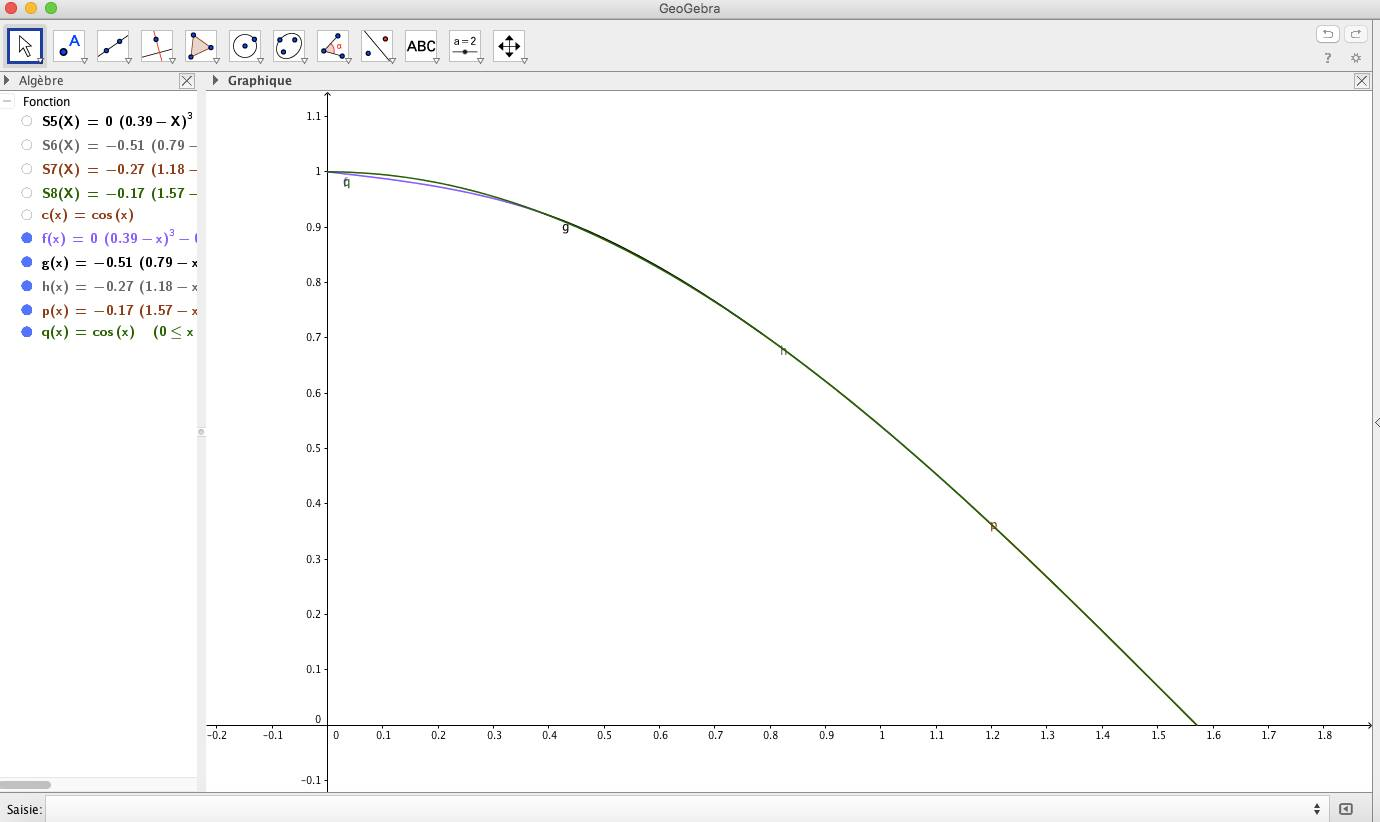
\includegraphics[width=0.5\textwidth]{FonctionCosinus.jpg}}
		\end{figure}
			\begin{figure}
			\putat{25}{-50}
				{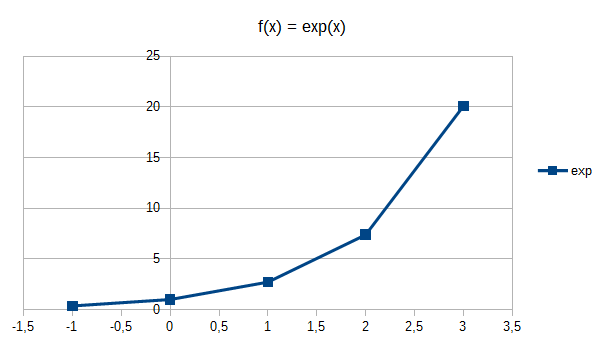
\includegraphics[width=0.5\textwidth]{FctExpExcel.png}}
			\end{figure}
    	\hyperlink{sommaire}{\beamerreturnbutton{Retour Sommaire}}
	\end{frame}
	
	
	
		
	\placelogotrue
	\section{Applications des splines cubiques}
		\subsection{Typographie}
	\begin{frame} 
		\frametitle{Typographie}
		\begin{alertblock}

 			- D\'eveloppement de l'informatique			
		\end{alertblock}
		\begin{figure}
			
\includegraphics[width=0.4\textwidth]{Typographie.png}
		\end{figure}
		\begin{alertblock}

 			- Disparition de la pixellisation par l'utilisation des interpolations par splines
 			\\
			- Mod\'elisation avec les logiciels de dessin tels que Geogebra et Paint
		\end{alertblock}
    	\hyperlink{sommaire}{\beamerreturnbutton{Retour Sommaire}}
	\end{frame}

	
	
	
	
	\placelogofalse
		\subsection{Les autres applications des interpolations par spline}
	\begin{frame}  
		\frametitle{Les autres applications des interpolations par spline}

		\begin{alertblock}
			{Nombreux domaines d'application des interpolations :}
				\begin{itemize}
				\item	A\'eronautique et automobile avec la F.A.O. (Fabrication Assist\'ee par Ordinateur)
				\item	Chimie, avec l'interpolation par fonctions splines restreintes
				\item	Imagerie m\'edicale
				\item	Le Taj Mahal 
				\end{itemize}
		\end{alertblock}
		
			\begin{figure}
			\putat{-160}{-45}
				{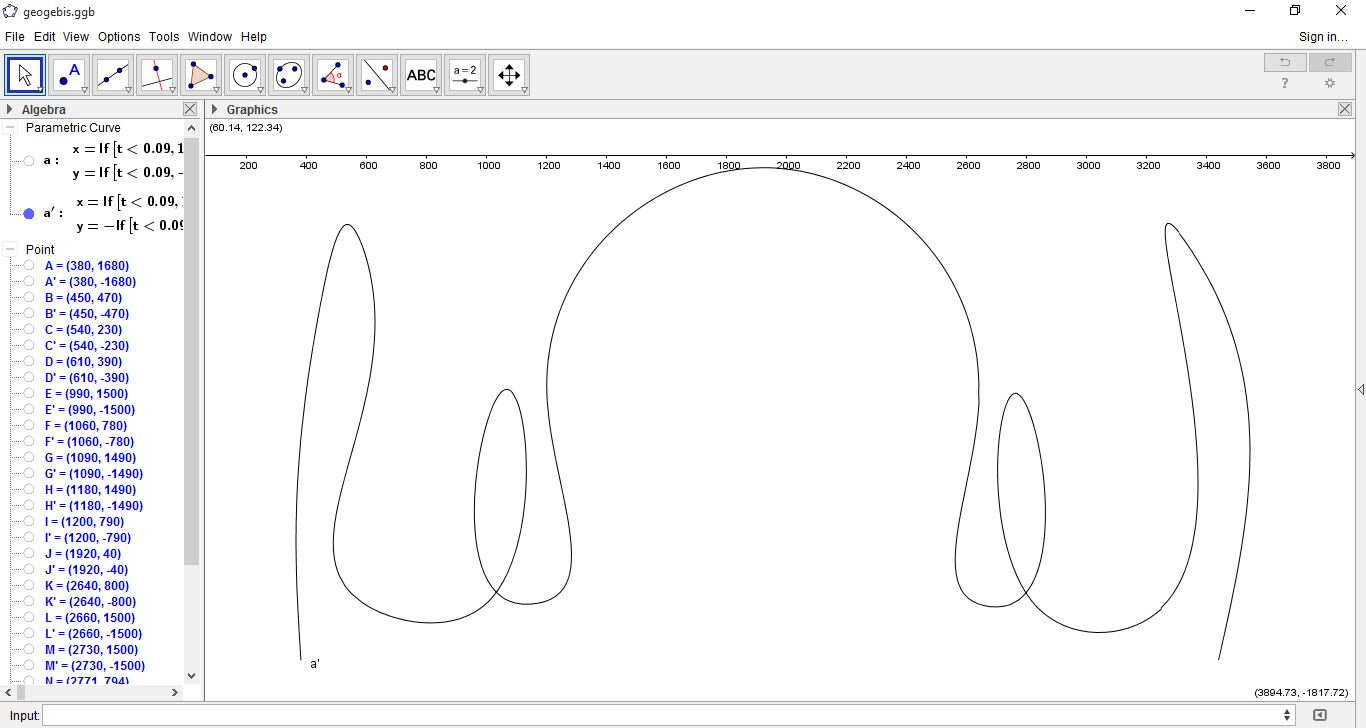
\includegraphics[width=0.43\textwidth]{GeogebraTajMahal.JPG}}
			\end{figure}
		
		
			\begin{figure}
			\putat{-10}{-10}
				{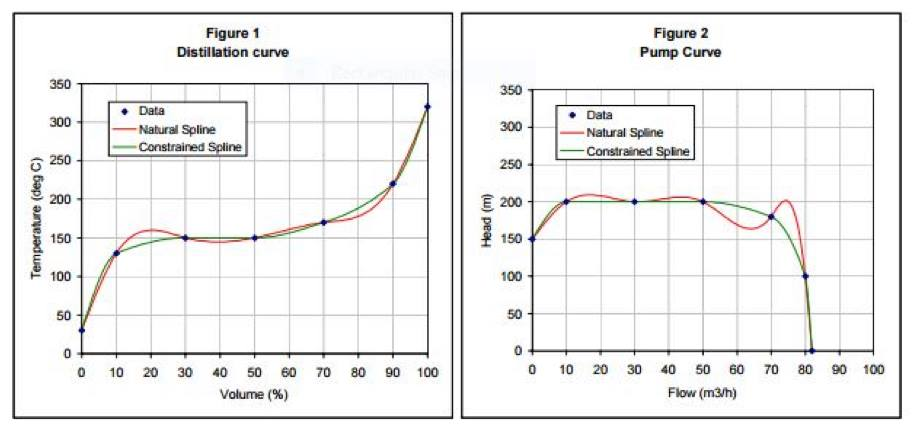
\includegraphics[width=0.6\textwidth]{SplineChimie.png}}
			\end{figure}
		
    	\hyperlink{sommaire}{\beamerreturnbutton{Retour Sommaire}}
	\end{frame}
	
	%\section{Conclusion}
	\begin{frame}
	
	
	\begin{center}
	\begin{large}
		CONCLUSION
	\end{large}
	\end{center} 
	
	\end{frame}
	

	\end{document}